\chapter{Implementcja translatora}
\section{Parser}
Istnieje ścisła zależność pomiędzy każdym typem języków w hierarchii Chomskiego, ich gramatykami i automatami rozpoznającymi napisy w tych językach.\cite{CHOMSKY1959}\cite{hopcroft_automaty}
\begin{center}
\begin{tabular}{|c|c|c|}
\hline
\textbf{Stopień w hierarchii} & \textbf{Gramatyka} & \textbf{Automat} \\ \hline
0 & Struktur frazowych (nieograniczona) & Maszyna Turinga \\ \hline
1 & Kontekstowa & Liniowo ograniczony\\ \hline
2 & Bezkontekstowa & Ze stosem\\ \hline
3 & Regularna & Skończenie stanowy\\ \hline
\end{tabular}
\end{center}

Dla automatycznej analizy składniowej są użyteczne zazwyczaj dwa dolne stopnie tej hierarchii. Analizę leksykalną przeprowadza się definiując tokeny z użyciem języków regularnych, (Chociaż napisanie efektywnego leksera jest daleko trudniejsze niż użycie biblioteki do tzw. ,,regexów'', zob. osiemdziesięciostronicowy rozdział trzeci w podręczniku\cite{DRAGON_BOOK}).

Samo egzystencjalne twierdzenie o istnieniu automatu ze stosem rozpoznającego język bezkontekstowy, niewielką jest pociechą dla piszącego jego translator – potrzebny jest konkretny sposób jego konstrukcji. Nie jest to zagadnienie trywialne i poświęcono mu wiele uwagi w pierwszych dekadach rozwoju języków wysokopoziomowych. W tekście tego rodzaju, nie jest możliwe choćby naszkicowanie kształtów wielkiego gmachu lingwistyki formalnej, ani nawet teorii parsingu. Powiedziane zostanie zaledwie tyle, by umotywować wybór narzędzia do analizy składniowej.

Istnieje kilka algorytmów konstrukcji automatu dokonującego rozbioru zdań w języku opisywanym zadaną gramatyką bezkontekstową. Automat taki nazywany bywa również parserem i miano ta odpowiada jego naturze – bo istotnie wydziela części (łac. - pars) zdania, konstruując drzewo składniowe, gdzie liśćmi są terminale, gałęziami symbole nieterminalne, a korzeniem symbol startowy (choć w praktyce najłatwiej stworzyć parser jedynie rozpoznajacy, czy dany napis należy do języka, czy nie, samo zachowanie parsera zawiera informację o strukturze składniowej zdania, lecz aby ją wydobyć i skonstruować drzewo, potrzebna jest dodatkowa praca).\cite{DRAGON_BOOK}
%[rysunek dodać przykładowy]

Najprościej wyjaśnić można działanie parsera rekursywnie zstępującego (recursive descent). Konstrukcja jego jest w zasadzie trywialna. Załóżmy, że mamy produkcje gramatyki:

\begin{lstlisting}[numbers=left]
instr: 'jeśli' wyr 'to' instr 'koniec';
instr: 'dopóki' wyr 'to' instr 'koniec';
instr: lista_instr;
lista_instr: instr ';' lista_istr;
lista_instr: |$\epsilon$|; (pusta prawa strona produkcji)
\end{lstlisting}

Wystarczy, że zaopatrzymy się w analizator leksykalny z funkcją nast(), która zwraca następny token, dopasuj(t), która konsumuje token t ze strumienia wejściowego, to możemy niemal wprost „przepisać” gramatykę na procedury parsera: (zaadaptowane z \cite[str.~70]{DRAGON_BOOK})

\begin{lstlisting}
void instr(){
	switch(nast())
	case 'jeśli': wyr(); dopasuj('to'); instr(); dopasuj('koniec'); break; 
            (zob. produkcję (1))
	case 'dopóki': wyr() dopasuj('to'); instr(); dopasuj('koniec'); break;
            (zob. produkcję (2))
	default : zgłoś("Błąd składnoiwy")
}
\end{lstlisting}
Dopasowujemy terminale, a dla nieterminali generujemy podprocedury odpowiadające produkcjom mającym dany symbol po lewej stronie.
Nie skonstruujemy wszak w ten sposób parsera wyrażeń arytmetycznych:
\lstset{escapechar=@,}
\begin{lstlisting}
Gramatyka: 
wyr: wyr * wyr| wyr + wyr;

Procedura parsera: 
void wyr()
{
    wyr(); '+' wyr()...
}
\end{lstlisting}
\lstset{escapechar=|,}
gdyż oznaczałoby to nieskończoną rekursję. (Rekursja lewostronna jest ogólnie zakazana dla parserów zstępujących, jeśli nie usunie się je przekształcając gramatykę.)

Podobnie działa tabelaryczny parser LL, z tą różnicą, że ma formę jawnego automatu ze stosem, a nie zbioru procedur. Istnieją różne odmiany algorytmu generacji zbioru stanów takich parserów – kanoniczne LL(k) są w stanie rozpoznawać szersze klasy języków (im dalej pozwala im się podglądać wprzód, choć rośnie wtedy rozmiar zbioru stanów), SLL z kolei słabszy jest nawet od LL(1), lecz bardzo łatwy w konstrukcji.\cite{DRAGON_BOOK}

Ograniczenie parsera rekursywnie schodzącego, lub LL da się do pewnego stopnia omijać i niwelować, jednakże dowiedziono\cite{Nijholt}, że klasa języków LL(k) – parsowanych od lewej do prawej strony, zstępująco (od symbolu startowego do terminali), jest węższa niż LR(k) – wstępujących.

Donald Knuth 1965 w swoim artykule „Parsowanie od lewej do prawej”\cite{TRANSLATION_FROM_LEFT_TO_RIGHT} przedstawił algorytm konstrukcji parsera LR – wstępującego – który jako pierwszy algorytm rozbioru posiadał gwarancję działania w czasie liniowym względem długości wejścia. Dostrzeżono powszechnie wielki potencjał w parserach LR,  choć ich tabele (zbiory stanów), nawet dla LR(2) - podglądającego co najwyżej dwa symbole wprzód - okazywały się zbyt obszerne względem dostępnej pamięci. Dość szybko, w roku 1969 de Remer zaproponował efektywny sposób ich kompresji\cite{LALR}. Ta odmiana algorytmu – LALR, została zastosowana w generatorze parserów yacc – gdyż generowanie tabel według algorytmów można zautomatyzować i programista musi wtedy stworzyć jedynie gramatykę, a narzędzie przekształci ją w parser. W 1975 Bell Labs zmieniło w swoim kompilatorze C parser na generowany przez yacc, w miejsce pisanego ręcznie rekursywnie schodzącego. Na długie lata generowane parsery LALR stały się standardem, a para uniksowych programów lex-yacc, podstawą zarówno wielu narzędzi – np. awk, jak i poważnych jezyków – perl.\cite{parsing_timeline_kegler}

Z powodu tej ugruntowanej pozycji LALR, wielkim zaskoczeniem dla postronnych mogła być decyzja projektu gcc, gdzie w 2006 roku wymieniono parser z powrotem na ręcznie pisany, rekursywnie schodzący.\cite{gcc_2006_release_note} Przyczyny tego „regresu” można dopatrywać się w zwiększonych wymaganiach użytkowników względem komunikatów o błędach. W ręcznie pisanym parserze, można umieścić dowolnie złożoną obsługę błędów. Zarządzanie zachowaniem generowanego parsera LR jest natomiast trudniejsze, oznacza manipulowanie stanem stosu symboli i odpowiednio dużej ilości niezbędnych poprawek, można stwierdzić, że prościej byłoby taki parser napisać ręcznie. Ponadto LR, będąc parserem wstępującym, nie posiada informacji, wewnątrz jakiego symbolu nieterminalnego znajduje się analizowana fraza, w przeciwieństwie do LL, który „schodzi” od symbolu startowego gramatyki przez kolejnie nieterminale. Ta sama własność, która pozwala LR rozpoznawać szerszą klasę języków, pozbawia go jednocześnie części informacji przydatnych w konstruowaniu zrozumiałych dla człowieka komunikatów o błędach.\cite{parsing_timeline_kegler}%[parsing timeline „LR fast but stupid”]

Teoretycznie jeszcze lepsze komunikaty może zapewnić parser działający wedle algorytmu Earleya\cite{EARLEY_1970}. W przeciwieństwie do LL i LR, rozpoznaje on wszystkie języki bezkontekstowe, również te niejednoznaczne, zwracając wszystkie możliwe rozbiory. Ceną za taką ogólność jest jednak wydajność. Oryginalny algorytm z roku 1970 roku miał złożoność pesymistyczną $O(n^2)$ i z tego powodu nie zyskał szerszej popularności, co zrozumiałe, ze względu ówczesne na ograniczenia sprzętowe. Joop Leo w 1991 zoptymalizował wszak jego działanie dla rekursji prawostronnych, uzyskując liniową złożoność dla gramatyk LR(k)\cite{JOOP_LEO_1991} (obejmujących większość gramatyk wykorzystywanych w praktyce\cite{parsing_timeline_kegler}), a w 2002 roku poprawiono drobny błąd pierwotnego algorytmu dla produkcji o zerowej długości\cite{AYCOCK_HORSPOOL_NIGEL_2002}. Wskutek tych ulepszeń, zmodyfikowany algorytm Earleya, ma praktyczną złożoność $O(n)$ dla całek klasy LR(k) – taką samą jak algorytm Knutha, i zwalnia do $O(n^2)$ dla niektórych dowolnych gramatyk bezkontekstowych.\cite{what_is_marpa_algorithm} W ostatnich latach więc zdobywa coraz większą popularność w zastosowaniach praktycznych, czego przykładem może być biblioteka nearley\cite{nearley}, albo generator parserów Marpa\cite{marpa_paper}\cite{marpa_page}.

Istnieją tez alternatywne podejścia – parsowanie Pratta wyrażeń z operatorami, któremu zawdzięczamy powszechne w specyfikacjach języków tabele z poziomami precedencji operatorów, czy inne podejście nieoparte na gramatykach Chomskiego – GEP. Rzeczywistość jest oczywiście dużo bardziej złożona, niż tu opisano i w praktycznych zastosowaniach mówi się również o LL(*), LR(*), GLR, LRR i wielu innych rozwiązaniach pośrednich.

Jednym z nich jest ANTLR. Teoretycznie jest predykcyjnym parserem rekursywnie schodzącym, lecz do wyboru ścieżki używa ATN (augmented translation networks – wzbogaconych sieci tłumaczeniowych) – konceptu właściwego początkowo parserowi GLR – wstepującemu, tutaj zastosowanymi dla analizatora zstępującego.\cite{PARR_2014}

Ogólnie procedura generowana przez antlr dla nieterminala instrukcji, analogicznego do poprzedniego przykładu wygląda następująco:
\lstset{
    escapechar=|,
    breaklines=true
}
\begin{lstlisting}
public final InstrukcjaContext |\textbf{instrukcja()}| throws RecognitionException {
    InstrukcjaContext _localctx = new InstrukcjaContext(_ctx, getState());
    enterRule(_localctx, 16, RULE_instrukcja);
    try {
        setState(143);
        _errHandler.sync(this);
        |\textbf{switch}| ( getInterpreter().|\textbf{adaptivePredict(\_input}|,5,_ctx) ) {
        case 1:
            enterOuterAlt(_localctx, 1);
            {
            setState(133);
            |\textbf{instrukcja\_wyboru();}|
            }
            break;
        case 2:
            enterOuterAlt(_localctx, 2);
            {
            setState(134);
            |\textbf{instrukcja\_petli();}|
            }
            break;
            ...
\end{lstlisting}
Działa więc on jak zwykły parser predykcyjny, nie używając jednak bezpośrednio podglądu tokenów, lecz skomplikowanego mechanizmu, generującego w locie automaty skończenie stanowe\cite{PARR_2014}. Teoretycznie charakteryzuje się pesymistyczną złożonością $O(n^4)$, lecz w praktyce generuje jedne z szybszych parserów i jest powszechnie stosowany. Autor tego tekstu, pracując nad projektami w Javie, zupełnie z pozoru niezwiązynymi z zagadnieniami parsingu, odnajdywał wielokrotnie antlr na listach zależności – używają go biblioteki do parsowania html, json i inne powszechnie wykorzystywane.

Jedną z najbardziej użytecznych cech antlr jest automatyczne przeprowadzanie niektórych przekształceń gramatyki, a w szczególności usuwania lewostronnej rekursji (gdy to możliwe), zachowując jednocześnie na potrzeby użytkownika oryginalne nieterminale. Widać to szczególnie wyraźnie w składni wyrażeń w przedrukowanej w poprzednim rozdziale gramatyce. (Tradycyjnie, konieczne byłoby rozbicie je na wiele nieterminali, analogicznie do gramatyki 4.2 na stronie 223 ,,Dragon Book''\cite{DRAGON_BOOK}.)

Ponadto antlr to posiada dobrze napisany oficjalny podręcznik\cite{Definitive_antlr_reference}, z wieloma przykładami w Javie. 

\subsection{Język implementacji - Java}
Antlr posiada wersje generujące kod w kilku językach, jednak dostępność przykładów i materiałów w Javie, była jednym z powodów jej wyboru jako języka implementacji kompilatora. Drugim było jej automatyczne zarządznie pamięcią, zdejmujące konieczność zwalniania mnogich węzłów różnych drzewiastych struktur wykorzystywanych przez translator. 

Pisanie kompilatora projektowanego języka w nim samym odrzuciłem, ze względu na wciąż trwający rozwój składni, brak automatycznego zarządzania pamięcią na tym etapie oraz oczywiście na ogromną ilość pracy którą należy włożyć w uzyskanie pierwszej wykonywalnej wersji translatora (co zostało opisane w przypadku Pascala, a nowszym przykładem może być język Go).

\section{Prototyp}
Sama idea języka z równoprawnymi punktami wejściowymi do procedur pojawiła się w moim umyśle na wiosnę roku 2022, gdy brałem udział w zajęciach z przedmiotu ,,Teoria kompilacji''. Udało mi się zachęcić dwie osoby w grupie projektowej do podjęcia tego pomysłu i w ten sposób, jako projekt zaliczeniowy, powstał program, który można by nazwać prototypem prezentowanego tutaj. Niestety, z przyczyn, które objaśnię poniżej, praktycznie żaden kod z prototypu nie znalazł się w bieżącej wersji, sam język też zmienił się dość wyraźnie.

\subsection{Założenia}
Prototyp opierał się na prostym założeniu. Miał generować kod w NASM (Netwide Assembler), jako zwyczajny tekst, który miał potem być tłumaczony poprzez sam program nasm do kodu wykonywalnego. Wspominane już problemy przydziału rejestrów, optymalizacji i wyboru instrukcji zupełnie pominięto, poprzez użycie jako architektury docelowej wąskiego podzbioru IA-32. W porównianiu z 64 bitową wersją, ma prostszą konwencję wywołań, wszystkie parametry procedur składa się na stos przed wykonaniem instrukcji call, podczas gdy w IA-64 (potocznie x86-64) kilka pierwszych parametrów przekazuje się w rejestrach, co zmusza do podjęcia problemu ich przydziału, czym tamten program w ogóle się nie zajmował - każde podwyrażenie po prostu zwracało wynik w rejestrze akumulatora (eax), co efektywnie eliminowało zagadnienie, za cenę fatalnej wydajności generowanego kodu. 

Korzyścią z generowania kodu w języku średniego poziomu, był sposób implementacji wielu punktów wejściowych do procedur - naturalny i analogiczny do wskazanego wcześniej, wykorzystywanego w asemblerach.

\subsection{Ograniczenia}
Ograniczenia takiej metody stały się jednak widoczne jeszcze w trakcie trwania tamtego projektu. Łatwo zobrazować je, obserwując kod generowany przez clanga (clang -S plik.c) dla prostej funkcji, na przykład dodającej dwie liczby, w jednym wypadku całkowite, w drugim wypadku zmiennoprzecinkowe:
\begin{center}
\begin{tabular}{|c | c|}
\hline
\begin{lstlisting}
int f(int a, int b)
{
    return a+b;
}
\end{lstlisting}
&
\begin{lstlisting}
double f(double a, double b)
{
    return a+b;
}
\end{lstlisting}
\\ \hline
\begin{lstlisting}
f:
	leal	(%rcx,%rdx), %eax
	retq
\end{lstlisting}
&
\begin{lstlisting}
f: 
	addsd	%xmm1, %xmm0
	retq
\end{lstlisting}
\\ \hline
\end{tabular}
\end{center}
Nawet prosty przypadek z liczbami całkowitymi może nas zaskoczyć, spodziewalibyśmy się instrukcji add, jednak najwyraźniej sprytne wyzyskanie adresowania pośredniego jest preferowane przez optymalizujący kompilator. W wersji zmiennoprzecinkowej z pozoru niewinne addsd okazuje sie być instrukcją wektorową - ,,Add Scalar Double Precision Floating-Point Values''\cite{ADDSD_instr} wymagająca rozszerzeń wektorowych SSE-2 w procesorze. 

Gdy zaczniemy uważniej czytać opisy takich instrukcji, nie umknie z pewnością zarówno ich mnogość, fakt używania osobnych rejestrów (i istnienie specjalnych instrukcji do przemieszczania danych pomiędzy nimi a rejestrami ogólnego przeznaczenia), jak i zalew drobnych szczegółów, chociażby konieczność wyrównania adresów do np. 16 bajtów dla instrukcji wektorowych. Karą za choćby drobne zaniedbanie podczas pracy na fizycznej maszynie, jest zazwyczaj gwałtowne zatrzymanie wykonywania programu, lub co gorsza doprowadzenie go do takiego stanu, że analiza post-mortem z użyciem debuggera nie wykazuje przyczyny. Podsumowując: efektywne użytkowanie współczesnej architektury CISC z pewnością nie jest zadaniem na miarę małego zespołu programistów. Narzędzia pokroju LLVM stają się koniecznością.

\subsection{Zastosowanie wzorca visitor w translatorze}
Wiele klasycznych przykładów, włączając to te z ,,Dragon Book''\cite{DRAGON_BOOK}, do fizycznej implementacji gramatyk atrybutowanych, używa akcji osadzonych w gramatyce. Terence Parr w podręczniku do antlr\cite{Definitive_antlr_reference} zauważa, że takie podejście ma swoje ograniczenia. Wychodząc poza krótkie gramatyki z dołączoną nieskomplikowaną semantyką (pokroju kalkulatora obliczającym wartości prostych wyrażeń), trudno utrzymać czytelność kodu. Gramatyka przetykana akcjami staje się mało czytelna, sam kod realizujący semantykę również. Można próbować ograniczać jego objętość, przesuwając większość logiki do procedur pomocniczych, jednak pewna jego część pozostać musi bardzo ściśle związana z gramatyką. Jako alternatywę, zmniejszającą ścisłe powiązanie pomiędzy realizacją parsera a kodem procedur semantycznych, proponuje Terence Parr zastosowanie jednego z dwóch wzorców projektowych - listener lub visitor. Antlr oprócz parsera generuje klasę BaseVisitor, która można rozszerzać i w ten sposób umieścić procedury semantyczne w osobnym pliku, wykonywane podczas jawnego przechodzenia drzewa rozbioru. Gramatyka pozostaje wówczas zwarta i czysta, pozbawiona akcji, a osobny plik określa akcje dla kolejnych symboli nieterminalnych. Dzięki temu rozdziałowi, gramatyka staje się zarówno czytelna, jak i zdatna do wykorzystania w niezmienionej formie do implementacji innych akcji. Na przykład, gdyby ktoś chciał napisać automatyczny formater do języka, mógłby użyć pierwotnego pliku z gramatyką, tworząc jedynie inne rozszerzenie klasy BaseVisitor.

Zachęcony tymi argumentami, użyłem wzorca visitor, lecz to samo w sobie okazał się niewystarczające. Większość istotnego kodu aplikacji stłoczyła się w jednej klasie, mimo wydzielania rozsądnych procedur pomocniczych. Część logiki deklaracji, sprawdzania typów i schematy generacji kodu musiały zwyczajnie mieć bezpośredni dostęp do drzewa rozbioru i nie dało się ich przenieść. Poważną przeszkoda okazało się również to, że drzewa rozbioru automatycznie produkowanego przez antlr4, w zasadzie nie można modyfikować, a przecież przekształcenia drzew są kluczowym mechanizmem optymalizującego kompilatora.

\section{Drzewa rozbioru a abstrakcyjne drzewa składniowe}
W literaturze oddziela się drzewa rozbioru (parse trees) od abstrakcyjnych drzew składniwych (abstract syntax trees, AST).\cite{DRAGON_BOOK} Drzewo rozbioru jest strukturą, która produkuje parser, odzwierciedla ono więc ono sposób zapisu języka, a ściślej, sposób w jaki ten zapis został zanalizowany. Abstrakcyjne drzewo składniowe z kolei ma reprezentować byty kryjące się pod tym zapisem. Najprościej pokazać tę różnicę na przykładzie prostego wyrażenia:

\begin{figure}[h]
    \centering
    \includesvg[width=0.5\linewidth]{images/ast_pt.svg}
    \caption{Drzewo rozbioru i abstrakcyjne drzewo składniowe}
\end{figure}

Nawiasy są jedynie własnością zapisu, pozwalającą ujednoznacznić hierarchię obliczeń, jak również odpowiednio pokierować procesem rozbioru. Gdy już poznaliśmy strukturę wyrażenia, stają się one zbędne (w innej formie zapisu, np. w notacji polskiej mogą być zupełnie nieobecne, a istniałaby napis o tej samej semantyce). W drzewie rozbioru znajdziemy przykładowo sygnaturę funkcji, nawiasy i listę instrukcji wewnątrz. Konceptualnie odpowiada im jednak obiekt reprezentujący funkcję, jej nazwę, blok jej kodu, lecz i jej zakres leksykalny z towarzyszącą tablicą symboli.

W tej wersji translatora zdecydowałem się na zaimplementowanie węzłów AST osobno, jako obiektów specjalnie zdefiniowanych w Javie klas. Wpierw parser tworzy drzewo składniowe. Przykładowo z takiego kodu źródłowego:

\begin{lstlisting}
printf(znak^, ...) -> całk32;
atoi(znak^) -> całk32;

proc{ zacznij program(całk argl, znak ^^ argw)->całk;
	całk i=0; dopóki(i<argl)
	{
    		całk w = atoi(argw[i]);
    		jeśli(w%3==0){printf("%x ", w);}
	}
}
\end{lstlisting}
powstaje drzewo rozbioru w formie przedstawionej na następnej stronie. (Rys. \ref{img_pt})

\begin{landscape}
\begin{figure}[p]
    \centering
        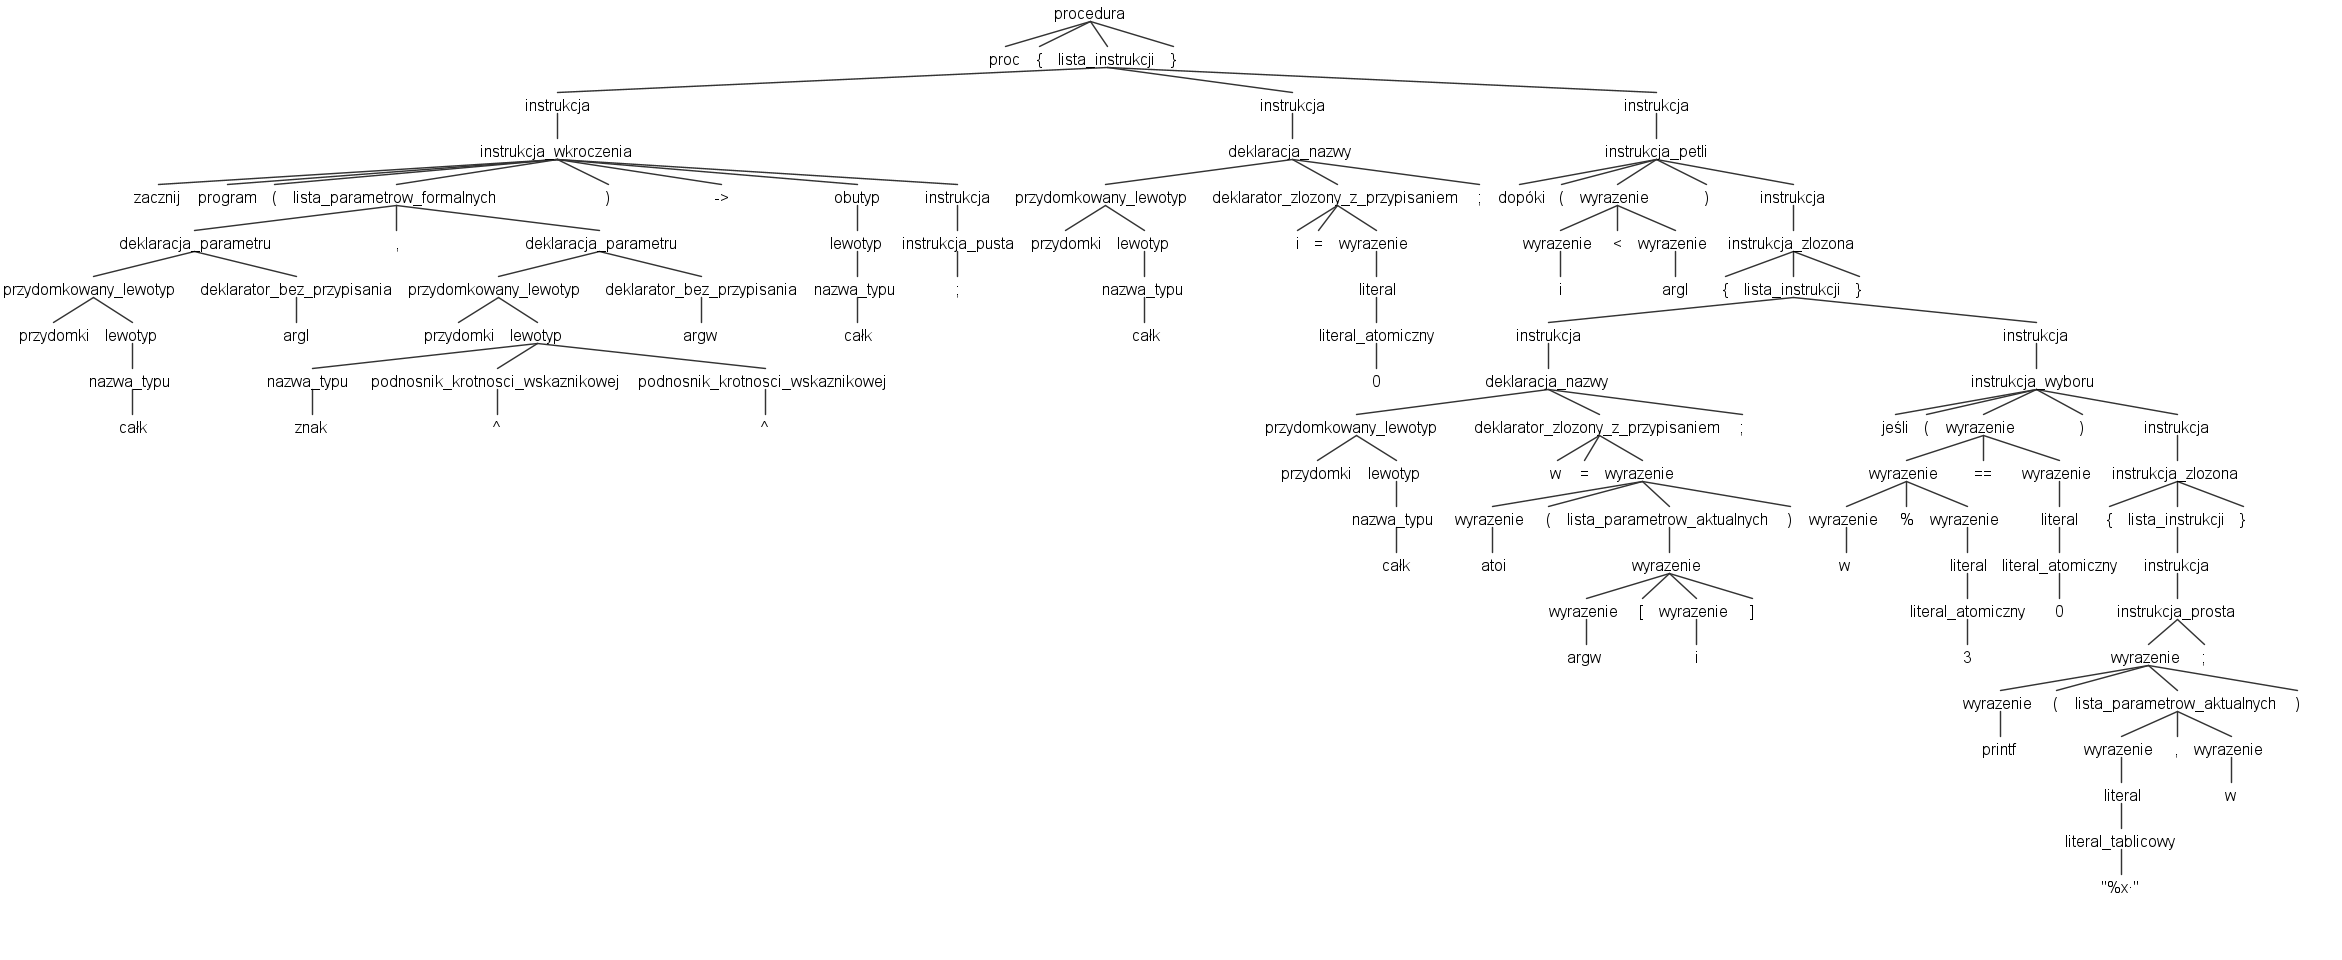
\includegraphics[width=\linewidth]{images/1.progmain/prezifelsePT1.png}
    \caption{Drzewo rozbioru}
    \label{img_pt}
\end{figure}
\end{landscape}

\begin{landscape}
\begin{figure}[p]
    \centering
    \includesvg[width=\linewidth]{images/1.progmain/prz.5.prezentacja_petla_if.ast.svg}
    \caption{Utworzone abstrakcyjne drzewo składniowe}
    \label{img_ast}
\end{figure}
\end{landscape}

\begin{landscape}
\begin{figure}[p]
    \centering
    \includesvg[width=\linewidth]{images/1.progmain/prz.5.prezentacja_petla_if.tpast.svg}
    \caption{Typowane drzewo składniowe}
    \label{img_tpast}
\end{figure}
\end{landscape}
\begin{figure}[H]
    \centering
    \includesvg[width=1.0\textwidth]{images/1.progmain/cfg1.svg}
    \caption{Postać pośrednia LLVM (narysowana w formie grafu przepływu sterowania)}
    \label{img:img_llvm_ctrl_flow}
    %(opt -passes="dot-cfg" -disable-output .\\prz.5.prezentacja_petla_if.ll)
\end{figure}
\newpage%bo rysunek uciekł w kosmos

Wywołuje się potem rekursywnie na w węzłach drzewa rozbioru rozmaite metody ,,visit''. Następuje wtedy przetworzenie deklaracji, wstawienie nazw do zasięgów oraz budowa abstrakcyjnego drzewa składniowego (Rys. \ref{img_ast}).

Kolejnym krokiem jest uruchomienie procedury sprawdzania typów. W jej toku obliczany jest typ każdego węzła i sprawdzane są odpowiednie ograniczenia równości typów. Wyrażenia, gdzie oblicza się adres a nie wartość (lwartości), np. lewe strony operatorów przypisania, są sprawdzane, aby upewnić się, że istotnie posiadają adres w pamięci (a nie są np. stałą). Niekiedy, trzeba wstawiać dodatkowe węzły konwersji, jeśli zezwalają na to reguły konwersji automatycznych, w przeciwnym wypadku trzeba zgłosić błąd. Błędy zawierają numer linii, ponieważ węzły AST zachowują informację o pozycjach w tekście źródłowym węzłów drzewa rozbioru, z których powstały. (Rys. \ref{img_tpast})

Po tych zabiegach, można wygenerować kod. W tym celu na węzłach AST wywołuje się rekursywnie rozmaite metody ,,generate'', które poprzez schematy translacji wywołujące odpowiednio funkcje LLVM C API, tworzą trzecie drzewo - postaci pośredniej LLVM (rys. \ref{img:img_llvm_ctrl_flow}) 
%\marginnote{Obrazek generuje się na innej stronie dlatego zamiast dwukropka należy podac odwołanie do obrazka}
%Rysunek przeniesiony wyżej, by był zaraz po drzewach składniowych

\section{Postać pośrednia LLVM}
Postać pośrednią LLVM zaprojektowano jako uniwersalną reprezentację, używaną zarówno przy kompilacji C jak i C++ w clang. Jej tekstową reprezentację można uzyskać wywołując program clang z przełącznikami ,,-S -emit-llvm''. Wydaje się ona być językiem pomiędzy C/C++ a asemblerem, uproszczonym, pozbawionym na przykład wszelkich automatycznych konwersji, traktującym wszystkie wskaźniki jednako, lecz z drugiej strony posiadając np. wyodrębnione pojęcie funkcji. Najlepiej jednak naturę LLVM IR przedstawia rys.\ref{img:img_llvm_ctrl_flow}, ponieważ LLVM IR stanowi w pierwszym rzędzie drzewiastą reprezentację w roboczej pamięci translatora.

Najwyższym w jej hierarchii jest moduł i zawierać on może wiele funkcji, każda funkcja zawiera listę bloków, a blok listę instrukcji. Każdy blok wszakże musi być ,,domknięty''(sealed), czyli kończyć się instrukcją skoku (warunkowego, bezwarunkowego, lub pośredniego), albo powrotu. Konstruuje się w ten sposób graf przepływu (control flow graph), który jest strukturą niezbędną do przeprowadzania dalszych analiz i optymalizacji.\cite{llvm_lang_ref}

Można zapisać LLVM IR w postaci tekstowej (plików .ll). Jak wspomniano, w przypadku kompilacji C można wywołać "clang -S -emit-llvm plik.c". Zaimplementowany w tej pracy kompilator z kolei wywołuje odpowiednią funkcję w LLVM C API. Dla omawianego powyżej programu, wygenerowana postać pośrednia przedstawia się następująco:

\begin{lstlisting}[
    basicstyle=\scriptsize
]
; ModuleID = 'src\test\java\pl\plpl\prz.5.prezentacja_petla_if'
source_filename = "src\\test\\java\\pl\\plpl\\prz.5.prezentacja_petla_if"

@"napis_%x _8:29-8:33" = global [4 x i8] c"%x \00"

declare i32 @printf(ptr, ...)

declare i32 @atoi(ptr)

define i64 @program(i64 %0, ptr %1) {
wejscie:
  %i = alloca i64, align 8
  %argw = alloca ptr, align 8
  %w = alloca i64, align 8
  %argl = alloca i64, align 8
  store i64 %0, ptr %argl, align 4
  store ptr %1, ptr %argw, align 8
  br label %drugiBlok

drugiBlok:                                        ; preds = %wejscie
  br label %"pierwszy_po_program_4:6-4:52"

"pierwszy_przeskakiwanyprogram_4:6-4:52":         ; No predecessors!
  br label %"pierwszy_po_program_4:6-4:52"

"pierwszy_po_program_4:6-4:52":                   ; preds = %"pierwszy_przeskakiwanyprogram_4:6-4:52", %drugiBlok
  store i64 0, ptr %i, align 4
  br label %"ptl_oblicznie_warunku_5:14-9:4"

"ptl_oblicznie_warunku_5:14-9:4":                 ; preds = %"j_poWarunkowej8:8-8:39", %"pierwszy_po_program_4:6-4:52"
  %i_wt = load i64, ptr %i, align 4
  %argl_wt = load i64, ptr %argl, align 4
  %"opProstai<" = icmp slt i64 %i_wt, %argl_wt
  %"opprostai_rozsz<" = zext i1 %"opProstai<" to i64
  %ptl__zwezenie_dla_warunku = icmp ne i64 %"opprostai_rozsz<", 0
  br i1 %ptl__zwezenie_dla_warunku, label %"pierwszyPetli_5:14-9:4", label %"poPetli_5:14-9:4"

"pierwszyPetli_5:14-9:4":                         ; preds = %"ptl_oblicznie_warunku_5:14-9:4"
  %argw_wt = load ptr, ptr %argw, align 8
  %i_wt1 = load i64, ptr %i, align 4
  %"ind_adr_7:22-7:28" = getelementptr inbounds ptr, ptr %argw_wt, i64 %i_wt1
  %"ind_wt_7:22-7:28" = load ptr, ptr %"ind_adr_7:22-7:28", align 8
  %"call_7:17-7:29" = call i32 @atoi(ptr %"ind_wt_7:22-7:28")
  %"sext7:17-7:29" = sext i32 %"call_7:17-7:29" to i64
  store i64 %"sext7:17-7:29", ptr %w, align 4
  %w_wt = load i64, ptr %w, align 4
  %"opProstai%" = srem i64 %w_wt, 3
  %"opProstai==" = icmp eq i64 %"opProstai%", 0
  %"opprostai_rozsz==" = zext i1 %"opProstai==" to i64
  %j__zwezenie_dla_warunku = icmp ne i64 %"opprostai_rozsz==", 0
  br i1 %j__zwezenie_dla_warunku, label %"j__gdyPrawdziwe_8:8-8:39", label %"j_poWarunkowej8:8-8:39"

"j__gdyPrawdziwe_8:8-8:39":                       ; preds = %"pierwszyPetli_5:14-9:4"
  %w_wt2 = load i64, ptr %w, align 4
  %"call_8:22-8:37" = call i32 (ptr, ...) @printf(ptr @"napis_%x _8:29-8:33", i64 %w_wt2)
  br label %"j_poWarunkowej8:8-8:39"

"j_poWarunkowej8:8-8:39":                         ; preds = %"j__gdyPrawdziwe_8:8-8:39", %"pierwszyPetli_5:14-9:4"
  br label %"ptl_oblicznie_warunku_5:14-9:4"

"poPetli_5:14-9:4":                               ; preds = %"ptl_oblicznie_warunku_5:14-9:4"
  ret i64 0
}

define i32 @main(i32 %0, ptr %1) {
main_plpl_entry:
  %argc_sext = sext i32 %0 to i64
  %wywolanie_f_program = call i64 @program(i64 %argc_sext, ptr %1)
  %ret_main_plpl = trunc i64 %wywolanie_f_program to i32
  ret i32 %ret_main_plpl
}

\end{lstlisting}

Wyraźnie widać, że nie jest to język przeznaczony do recepcji przez osoby postronne. Poleganie na jego tekstowej postaci może okazać się zgubne, ponieważ sam LLVM ulega ciągłym przemianom i kod pośredni, jako format wewnętrzny, niezwiązany żadnym standardem zmienia się z czasem. Sama postać tekstowa jest również niedostatecznie udokumentowana i według mnie zrozumienie jej bez wcześniejszej znajomości mechanizmów LLVM i skuteczne użycie jest w zasadzie niemożliwe. Z kolei API jest wytłumaczone szczegółowo i przystępnie na przykładzie w znakomitym samouczku rozwijanym przez twórców LLVM\cite{kalleidoscope}, choć w moim wypadku pożyteczny okazał się również osobny podręcznik.\cite{llvm_nacke_textbook}

Podstawowym punktem odniesienia  jest oczywiście oficjalna dokumentacja\cite{llvm_lang_ref}. Wyczerpująco opisuje ona wszystkie istotne aspekty funkcjonowania tego systemu. Jedynym zastrzeżeniem, jakie autor tej pracy jest w stanie wobec niej wysunąć, jest to, że z biegiem czasu, powiększyła się znacznie o opisy mnogich specjalistycznych instrukcji, co czyni z niej bardzo długi dokument i zaciemnia jego strukturę. Piszący te słowa bardzo skorzystał, gdy trafił omyłkowo na starszą wersję dokumentacji, wielokroć krótszą, co eksponowało podstawowe elementy języka i systemu typów.

\section{Wybrane schematy translacji}
Zdecydowałem się na przedrukowanie tutaj niektórych schematów translacji w całości, żeby pokazać charakter interfejsu programistycznego LLVM i moją propozycję jego użycia w Javie (korzystając z JNI). Teksty te mogą się również okazać przydatne dla osoby, która znalazłaby się w sytuacji podobnej do mojej, potrzebując napisać takie schematy, dysponując jednocześnie dość szczupłym zbiorem przykładów, dostępnych w Sieci.

Schemat dla węzła ,,OperacjiProstej'' zawiera w zasadzie całą prostą arytmetykę.

\begin{lstlisting}[basicstyle=\scriptsize]
    public LLVMValueRef _generuj(LLVMContextRef c, LLVMValueRef func, LLVMBuilderRef builder, KontekstGeneracji kg){
        if(lewe.typ() == null || (!lewe.typ().równyFunkcjonalnie(prawe.typ()))){
            throw new WewnętrznyBłąd(String.format("OpProsta:nierówne typy: %s vs %s", lewe.typ(), prawe.typ()));
        }
        LLVMValueRef lewyrejestr = lewe.generuj(c, func, builder, kg);
        LLVMValueRef prawyrejestr = prawe.generuj(c, func, builder, kg);
        if(lewe.typ().jestWskaźnikiem()){
            return switch (opkod){
                case "==" -> LLVMBuildZExt(builder, LLVMBuildICmp(builder, LLVMIntEQ, lewyrejestr, prawyrejestr, "opProstap=="), reprTypuLogicznego(c) , "opprostap_rozsz==");
                case "!=" -> LLVMBuildZExt(builder, LLVMBuildICmp(builder, LLVMIntNE, lewyrejestr, prawyrejestr, "opProstap!="), reprTypuLogicznego(c) , "opprostap_rozsz!=");
                default -> throw new TODOException("Nieznany operand dla wskaźnika:"+opkod);
            };
        }
        if(!lewe.typ().jestAtomiczny()){ throw new TODOException("OpProsta:TylkoAtomiczne!"); }
        if(lewe.typ().jestCałkowity()){
            return switch (opkod) {
                case "+" -> LLVMBuildAdd(builder, lewyrejestr, prawyrejestr, "opProstai+");
                case "-" -> LLVMBuildSub(builder, lewyrejestr, prawyrejestr, "opProstai-");
                case "*" -> LLVMBuildMul(builder, lewyrejestr, prawyrejestr, "opProstai*");
                case "/" -> LLVMBuildSDiv(builder, lewyrejestr, prawyrejestr, "opProstai/");
                case "%" -> LLVMBuildSRem(builder, lewyrejestr, prawyrejestr, "opProstai%");
                case "==" -> LLVMBuildZExt(builder, LLVMBuildICmp(builder, LLVMIntEQ, lewyrejestr, prawyrejestr, "opProstai=="), reprTypuLogicznego(c) , "opprostai_rozsz==");
                case "!=" -> LLVMBuildZExt(builder, LLVMBuildICmp(builder, LLVMIntNE, lewyrejestr, prawyrejestr, "opProstai!="), reprTypuLogicznego(c) , "opprostai_rozsz!=");
                case ">" -> LLVMBuildZExt(builder, LLVMBuildICmp(builder, LLVMIntSGT, lewyrejestr, prawyrejestr, "opProstai>"), reprTypuLogicznego(c) , "opprostai_rozsz>");
                case ">=" -> LLVMBuildZExt(builder, LLVMBuildICmp(builder, LLVMIntSGE, lewyrejestr, prawyrejestr, "opProstai>="), reprTypuLogicznego(c) , "opprostai_rozsz>=");
                case "<" -> LLVMBuildZExt(builder, LLVMBuildICmp(builder, LLVMIntSLT, lewyrejestr, prawyrejestr, "opProstai<"), reprTypuLogicznego(c) , "opprostai_rozsz<");
                case "<=" -> LLVMBuildZExt(builder, LLVMBuildICmp(builder, LLVMIntSLE, lewyrejestr, prawyrejestr, "opProstai<="), reprTypuLogicznego(c) , "opprostai_rozsz<=");
                case "&&" -> LLVMBuildZExt(builder,
                                LLVMBuildAnd(builder,
                                        LLVMBuildTruncOrBitCast(builder, lewyrejestr, LLVMInt1TypeInContext(c), "&&ltrunc"),
                                        LLVMBuildTruncOrBitCast(builder, prawyrejestr, LLVMInt1TypeInContext(c), "&&rtrunc"),
                                    "&&and"),
                                reprTypuLogicznego(c), "&&zext");
                case "||" -> LLVMBuildZExt(builder,
                        LLVMBuildOr(builder,
                                LLVMBuildTruncOrBitCast(builder, lewyrejestr, LLVMInt1TypeInContext(c), "||ltrunc"),
                                LLVMBuildTruncOrBitCast(builder, prawyrejestr, LLVMInt1TypeInContext(c), "||rtrunc"),
                                "||or"),
                        reprTypuLogicznego(c), "||zext");
                default -> throw new TODOException("Nieznany operand całkowity:"+opkod);
            };
        }
        if(lewe.typ().jestZmiennoiprzecinkowy()) {
            return switch (opkod) {
                case "+" -> LLVMBuildFAdd(builder, lewyrejestr, prawyrejestr, "opProstaf+");
                case "-" -> LLVMBuildFSub(builder, lewyrejestr, prawyrejestr, "opProstaf-");
                case "*" -> LLVMBuildFMul(builder, lewyrejestr, prawyrejestr, "opProstaf*");
                case "/" -> LLVMBuildFDiv(builder, lewyrejestr, prawyrejestr, "opProstaf/");
                case "==" -> LLVMBuildZExt(builder, LLVMBuildFCmp(builder, LLVMRealOEQ, lewyrejestr, prawyrejestr, "opProstaf=="), reprTypuLogicznego(c) , "opprostaf_rozsz==");
                case "!=" -> LLVMBuildZExt(builder, LLVMBuildFCmp(builder, LLVMRealONE, lewyrejestr, prawyrejestr, "opProstaf!="), reprTypuLogicznego(c) , "opprostaf_rozsz!=");
                case ">" -> LLVMBuildZExt(builder, LLVMBuildFCmp(builder, LLVMRealOGT, lewyrejestr, prawyrejestr, "opProstaf>"), reprTypuLogicznego(c) , "opprostaf_rozsz>");
                case ">=" -> LLVMBuildZExt(builder, LLVMBuildFCmp(builder, LLVMRealOGE, lewyrejestr, prawyrejestr, "opProstaf>="), reprTypuLogicznego(c) , "opprostaf_rozsz>=");
                case "<" -> LLVMBuildZExt(builder, LLVMBuildFCmp(builder, LLVMRealOLT, lewyrejestr, prawyrejestr, "opProstaf<"), reprTypuLogicznego(c) , "opprostaf_rozsz<");
                case "<=" -> LLVMBuildZExt(builder, LLVMBuildFCmp(builder, LLVMRealOLE, lewyrejestr, prawyrejestr, "opProstaf<="), reprTypuLogicznego(c) , "opprostaf_rozsz<=");
                default -> throw new TODOException("Nieznany operand zmiennoprzecinkowy:"+opkod);
            };
        }
        kg.jk.katastrofa("Brak zdefiniowanej operacji prostej dla operandów typu: "+lewe.typ(), this.msc); return null;
    } 
\end{lstlisting}
Schemat dla pętli pokazuje, że o ile nie zadba się o odpowiednie ułożenie bloków, to schemat wparwdzie będzie działał, lecz zrzucony do pliku tekst postacji pośredniej będzie dl człowieka nieczytelny.
\lstset{
    escapechar=`,
    breaklines=true
}
\begin{lstlisting}[basicstyle=\scriptsize]
/*  ------>:obliczanie_warunku
    |       ...
    ^       %wyr_warunku = icmp ...
    |       br i1 %wyr_warunku, label %pierwszy_pętli, label %po_pętli
    |                                   |                       |
    ^   |--------------------------------                       |
    | |-+--------------------------------------------------------
    | | |-->:pierwszy_petli
    | V     ...
    ^ |     ...
    | |     ...
    | V     (:jakis_ostatni_pętli)?
    | |     ....
    --+---<-br %obliczanie_warunku
      |
      |---->:po_pętli
            ...
*/
    @Override
    public LLVMValueRef _generuj(LLVMContextRef c, LLVMValueRef func, LLVMBuilderRef builder, KontekstGeneracji kg) {
        sprawdźBlok(builder);
        //pętla ma skakać do początku obliczania warunku za każdym razem, więc potrzebujemy wstawić nowy blok, dodac skok bezwarunkowy z ostatniego do tego nwego.
        LLVMBasicBlockRef oblicznieWarunku = LLVMAppendBasicBlockInContext(c, func, "ptl_oblicznie_warunku_"+msc);
        LLVMMoveBasicBlockAfter(oblicznieWarunku, LLVMGetInsertBlock(builder));//na prawdziwym końcu funkcji coś może być już dołozone przez węzły wyżej
        LLVMBuildBr(builder, oblicznieWarunku);
        LLVMPositionBuilderAtEnd(builder, oblicznieWarunku);

        LLVMValueRef liczbaWarunku = warunek.generuj(c, func, builder, kg); sprawdźBlok(builder);
        assert liczbaWarunku != null;
        LLVMValueRef wyrWarunku = LLVMBuildICmp(builder, LLVMIntNE, liczbaWarunku, zeroTypuLogicznego(c), "ptl__zwezenie_dla_warunku");

        LLVMBasicBlockRef pierwszyWPętli = LLVMAppendBasicBlockInContext(c, func, "pierwszyPetli_"+msc);
        LLVMMoveBasicBlockAfter(pierwszyWPętli, oblicznieWarunku);//na prawdziwym końcu funkcji coś może być już dołozone przez węzły wyżej

        //Potrzebujemy referencji do bloku po pętli, by można było użyć break w środku pętli
        LLVMBasicBlockRef poPętli = LLVMAppendBasicBlockInContext(c, func, "poPetli_"+msc);
        LLVMMoveBasicBlockAfter(poPętli, pierwszyWPętli);

        LLVMBuildCondBr(builder, wyrWarunku, pierwszyWPętli, poPętli);

        //piszemy ciało pętli
        LLVMPositionBuilderAtEnd(builder, pierwszyWPętli);
        kg.stosPętli.push(new Etykietki(pierwszyWPętli, poPętli));//żeby break i continue miały się do czego odwoływać

        ciało.generuj(c, func, builder, kg); sprawdźBlok(builder);

        kg.stosPętli.pop();

        //domykamy pierwszyWPętli/któregos z jego następników
        LLVMBuildBr(builder, oblicznieWarunku);
        //przenosimy się za pętlę
        LLVMPositionBuilderAtEnd(builder, poPętli); sprawdźBlok(builder);
        return null;
    }
\end{lstlisting}

Schematy dla instrukcji warunkowych, wywołań są w zasadzie podobne i z racji częstego opisywania w literaturze, nie będą już cytowane.
\newpage

\section{Weryfikacja generacji kodu}
Oczekuje się od kompilatorów daleko większej niezawodności niż od ,,zwykłych'' aplikacji\cite{waite_goos}. Użytkownik języka nie zna zazwyczaj programu kompilatora i nie orientuje się szczegółowo w jego działaniu. Ostatnią rzeczą, jakiej spodziewa się programista języka wysokiego poziomu, próbując naprawić błąd w swym programie, jest defekt samego kompilatora. Z powodu tak dużej odpowiedzialności, w konstrukcji kompilatorów stawia się wysokie wymagania jakościowe i jednym ze sposobów ich wypełnienia są z pewnością szerokie testy, w szczególności automatyczne.

\subsection{Testy jednostkowe i wizualna reprezentacja AST}
Stworzenie przydatnych testów jednostkowych, napotkało w tym projekcie dwa zasadnicze problemy. Po pierwsze, wynikiem wielu powszechnych operacji są drzewa, a Java nie ma wbudowanego dopasowywania struktur (pattern matching), co czyni każdy kod sprawdzający strukturę drzewa bardzo nieczytelnym i kosztownym w utrzymaniu. Dodatkowo, w większości wypadków wymagany jest szerszy kontekst. Wewnątrz autorskiego kodu analizy semantycznej, da się utworzyć sztuczny kontekst, na potrzeby testów, choć jego odrębność, może negować całe przedsięwzięcie i czyni je kosztownym. Z kolei, wywołań API LLVM nie da się testować osobno - nie można utworzyć bloku, nie mając funkcji, funkcji nie mając modułu, a modułu bez utworzenia kontekstu LLVM.

W związku z tym, klasyczne testy jednostkowe znalazły jedynie ograniczone zastosowanie, np. przy testowaniu działania wyrażeń określających typ, gdzie da się wywołać parser przyjmując inny symbol startowy i sprawdzić równość wygenerowanego typu z oczekiwanym. O wiele bardziej użyteczne, zwłaszcza na etapie instensywnego rozwoju programu, było wizualne sprawdzanie generowanych drzew, przy pomocy prezentowanych powyżej diagramów AST. Każdy węzeł drzewa zaopatrzyłem w metodę zwracającą jego reprezentację w języku opisu grafów DOT, programu graphviz, który to program jest następnie wywoływany na rekursywnie zbudowanej reprezentacji, celem wygenerowania obrazka wektorowego (svg). Tekstowe przedstawienia AST stają się szybko nieczytelne już dla małych przykładów, a graficzna reprezentacja zawiera większość istotnej informacji i umożliwiają wizualną kontrolę dużo bardziej rozbudowanych konstrukcji. Zamieszczone wcześniej przykłady drzew składniowych - rys. \ref{img_ast}, \ref{img_tpast} były przykładami takich reprezentacji, bezpośrednio zaczerpniętymi z testów.

\subsection{Testy aplikacyjne - działające programy}
Oczywiście ostatecznym testem jest skompilowanie programu i sprawdzenie, czy wynikowy obraz wykonywalny, po uruchomieniu działa zgodnie z oczekiwaniami (choć to ostatnie można w praktyce sprawdzić jedynie dla bardzo prostych programów, bowiem przestrzeń możliwych wejść i wyjść rośnie bardzo szybko wraz ze złożonością kodu źródłowego). Drugim rodzajem testu, wielokroć prostszym do automatyzacji jest próba skompilowania programu błędnego i sprawdzenie, czy translator wygenerował odpowiednie komunikaty.

Do tego ostatniego celu uznałem uruchamianie programu kompilatora z zewnątrz za zbyteczne, utworzyłem osobny sposób wywołania kompilatora, z samej Javy, na zasadzie przypominającej API. Dzięki temu, poruszając się w środowisko Javy, test taki, zamiast przetwarzać tekst błędów, może sprawdzić równość i strukturę samych obiektów wygenerowanych zdarzeń, co pomija etap parsowania wyjścia samego kompilatora.

Udało mi się uzyskać zbiór programów testujących najważniejsze aspekty funkcjonowania translatora i błędy, które może zgłosić. Jednym z najistotniejszych celów utrzymywania zbioru takich testów, jest oczywiście testowanie regresyjne - aby zmiana w kodzie translatora ,,psująca'' coś, odzwierciedliła się natychmiast w automatycznych testach. Z pewnym zadowoleniem stwierdzam, że zbiór testów w tym projekcie już zaczął pełnić taką funkcję, pomimo braku pełnej automatyzacji testów pierwszego rodzaju.
%tu wrzucić jakieś przykłady uruchomionych programów????

\subsection{Weryfikacja poprawności generowanego obrazu wykonywalnego}
Dla niemal każdego programu, poza najbardziej trywialnymi, nie sposób przetestować wszystkich możliwych kombinacji wejść Użycie zaś programu typu \textit{fuzzer} wykracza poza zakres tej pracy, zresztą i tak generują one jedynie probabilistyczną próbkę przestrzeni napisów wejściowych. Ażeby skontrolować działanie całego procesu translacji, trzeba zatem przyjrzeć się również jego rzeczywistemu efektowi - obrazowi binarnemu. Dość łatwo uzyskać kod asemblerowy - wystarczy skompilować za pomocą clanga wygenerowany plik.ll z przełącznikiem -S, Dla poprzednio omawianego programu pełny wynik przedstawia się następująco:

\begin{lstlisting}[basicstyle=\scriptsize]
	.text
	.def	@feat.00;
	.scl	3;
	.type	0;
	.endef
	.globl	@feat.00
.set @feat.00, 0
	.file	"prz.5.prezentacja_petla_if"
	.def	program;
	.scl	2;
	.type	32;
	.endef
	.globl	program                         # -- Begin function program
	.p2align	4, 0x90
program:                                # @program
.seh_proc program
# %bb.0:                                # %wejscie
	subq	$72, %rsp
	.seh_stackalloc 72
	.seh_endprologue
	movq	%rcx, 40(%rsp)
	movq	%rdx, 56(%rsp)
# %bb.1:                                # %drugiBlok
	jmp	.LBB0_2
.LBB0_2:                                # %"pierwszy_po_program_4:6-4:52"
	movq	$0, 64(%rsp)
.LBB0_3:                                # %"ptl_oblicznie_warunku_5:14-9:4"
                                        # =>This Inner Loop Header: Depth=1
	movq	64(%rsp), %rax
	cmpq	40(%rsp), %rax
	setl	%al
	andb	$1, %al
	movzbl	%al, %eax
                                        # kill: def $rax killed $eax
	cmpq	$0, %rax
	je	.LBB0_7
# %bb.4:                                # %"pierwszyPetli_5:14-9:4"
                                        #   in Loop: Header=BB0_3 Depth=1
	movq	56(%rsp), %rax
	movq	64(%rsp), %rcx
	movq	(%rax,%rcx,8), %rcx
	callq	atoi
	cltq
	movq	%rax, 48(%rsp)
	movq	48(%rsp), %rax
	movl	$3, %ecx
	cqto
	idivq	%rcx
	cmpq	$0, %rdx
	sete	%al
	andb	$1, %al
	movzbl	%al, %eax
                                        # kill: def $rax killed $eax
	cmpq	$0, %rax
	je	.LBB0_6
# %bb.5:                                # %"j__gdyPrawdziwe_8:8-8:39"
                                        #   in Loop: Header=BB0_3 Depth=1
	movq	48(%rsp), %rdx
	leaq	"napis_%x _8:29-8:33"(%rip), %rcx
	callq	printf
.LBB0_6:                                # %"j_poWarunkowej8:8-8:39"
                                        #   in Loop: Header=BB0_3 Depth=1
	jmp	.LBB0_3
.LBB0_7:                                # %"poPetli_5:14-9:4"
	xorl	%eax, %eax
                                        # kill: def $rax killed $eax
	addq	$72, %rsp
	retq
	.seh_endproc
                                        # -- End function
	.def	main;
	.scl	2;
	.type	32;
	.endef
	.globl	main                            # -- Begin function main
	.p2align	4, 0x90
main:                                   # @main
.seh_proc main
# %bb.0:                                # %main_plpl_entry
	subq	$40, %rsp
	.seh_stackalloc 40
	.seh_endprologue
	movslq	%ecx, %rcx
	callq	program
                                        # kill: def $eax killed $eax killed $rax
	nop
	addq	$40, %rsp
	retq
	.seh_endproc
                                        # -- End function
	.data
	.globl	"napis_%x _8:29-8:33"           # @"napis_%x _8:29-8:33"
"napis_%x _8:29-8:33":
	.asciz	"%x "

	.addrsig
	.addrsig_sym printf
	.addrsig_sym atoi
	.addrsig_sym program
	.addrsig_sym "napis_%x _8:29-8:33"

\end{lstlisting}
Kod wygenerowany przez automat nie byłby miłą lekturą nawet dla doświadczonego programisty asemblerowego, a jak juz powiedziano na początku tego tekstu, znajomość asemblera na takim poziomie, by przeczytać powyższy wydruk i orzec z niewzruszoną pewnością o jego poprawności (lub niepoprawności), jako przekładu kodu źródłowego, to rzadka w dzisiejszych czasach umiejętność. Na szczęście istnieje prostszy sposób na weryfikację, i to nie sztucznie wygenerowanego asemblera, lecz bezpośrednio obrazu bianrnego, wyprodukowanego przez llvm (pliku .o, lub po konsolidacji, w zależności od systemu ELF lub EXE).

\subsection{Dekompilator Ghidra}
Amerykańska Agencja Bezpieczeństwa Narodowego oddała wielką przysługę postronnym, udostępniając za darmo jedno ze swych narzędzi - dekompilator Ghidra.\cite{ghidra}. Program tego rodzaju analizuje obraz wykonywalny i próbuje odtworzyć kod w języku wysokiego poziomu. Nie jest to oczywiście możliwe całkowicie - proces kompilacji jest stratną konwersją na wielu etapach, jednak interfejsy binarne, konwersje wywołań są na tyle blisko języka C, że można próbować częściowo go odtworzyć. 

Rekonstrukcja taka, pozbawiona będzie wszak wielu informacji, przede wszystkim nazw zmiennych, gdy pełne tablice symboli nie są obecne, co jest częstym zwyczajem podczas zwyczajnej kompilacji (nie sprofilowanej do debugowania). Osoba podejmująca się inżynierii wstecznej takiego obrazu, musi wtedy sama wydedukować przeznaczenie poszczególnych zmiennych i nadać im przypuszczalne nazwy.

Poniżej znajduje się zrzut ekranu, pokazujący efekt zastosowania Ghidry na obrazie binarnym omawianego programu.
\begin{figure}[h]
    \centering
    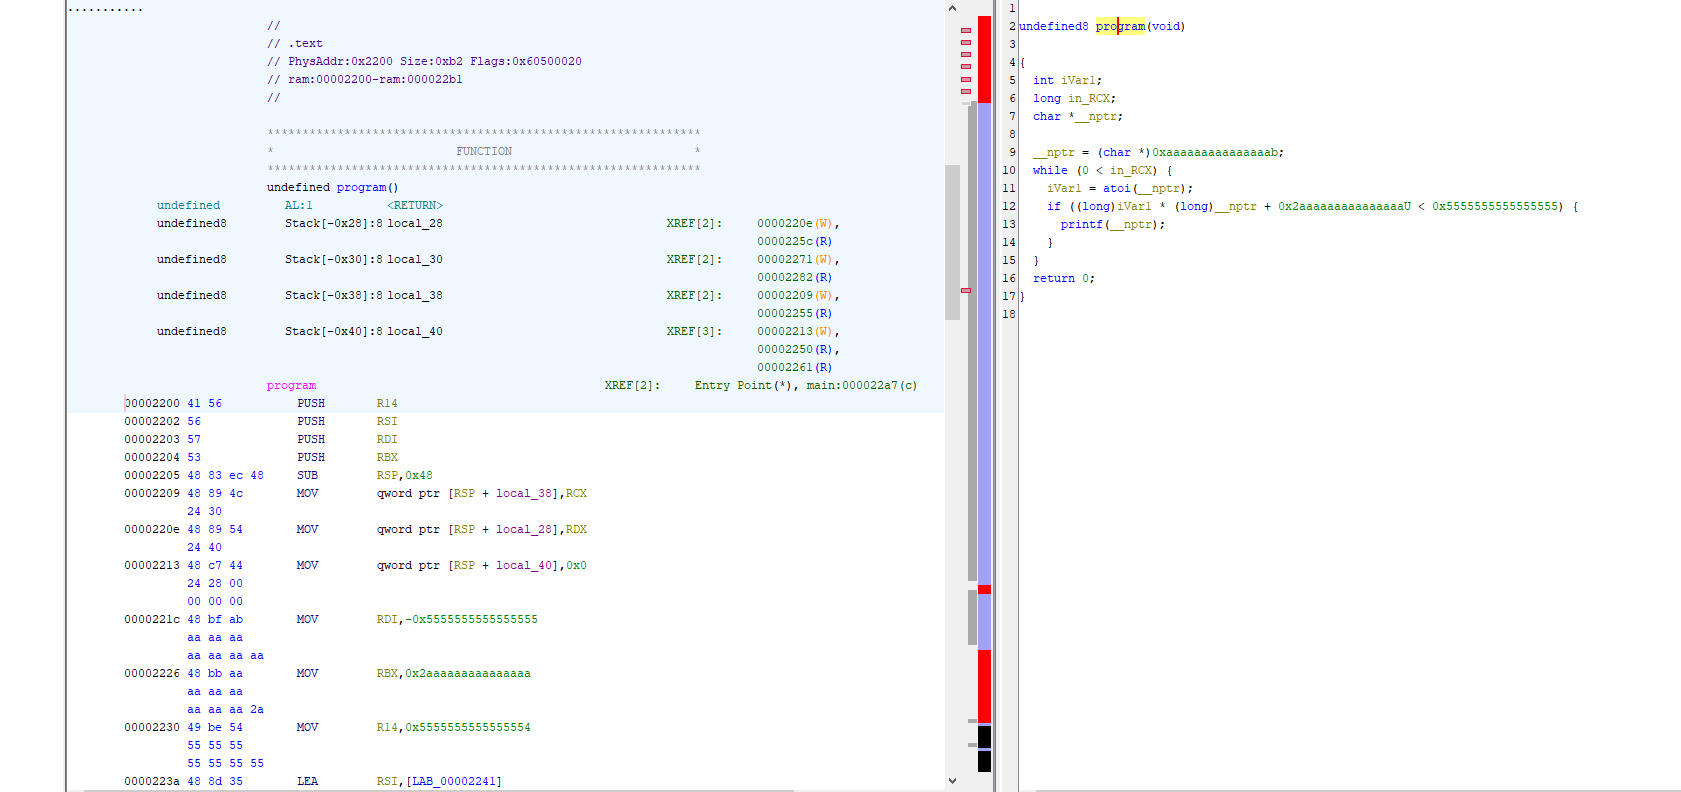
\includegraphics[width=1.3\textwidth]{images/1.progmain/ghidra1.png}
    \caption{Widok dekompilacji w programie GHIDRA}
\end{figure}

W lewym panelu znajduje się zdesamblewany kod, odpowiadający zamieszczonemu powyżej (Ghidra używa wszak składni Intela, różnej od GNU ASM, produkowanej domyślnie przez clanga). Po prawej stronie widnieje przypuszczalna rekonstrukcja programu w języku C. Poprawnie zrekonstruowano funkcję ,,program'' (akurat publiczne symbole zawsze znajdują się w obrazach), i ewidentnie zawiera ona pętlę i warunek, w układzie odpowiadającym kodowi źródłowemu. 

Za artefakty w postaci nieoczekiwanych stałych, oraz niepełnego wywołania wariadycznej funkcji printf, można obarczyć konwencję wywołań cdecl na IA-64, gdzie pierwsze argumenty funkcji znajdują się w rejestrach i dekompilator boryka się z właściwą ich interpretacją.
Niemniej jednak zweryfikowaliśmy, że cała maszyneria translatora istotnie działa i produkuje odpowiadający programowi źródłowemu, dość zgrabny kod, z pewnością nie ,,rażąco nieefektywny''.

\section{Sposób translacji wielokrotnych punktów wejściowych}
W tym miejscu wywodu pozostaje już tylko jeden punkt do objaśnienia - jak w przedstawionym stosie technologicznym zaimplementowano translację wielokrotnych punktów wejściowych. W prototypie, operując asemblerem, można było swobodnie rozsadzić zwyczajową strukturę kodu funkcji, umieszczając w jednej sekcji kodu kilka wołanych symboli. LLVM jednak operuje już wszak na podstawowym poziomie pojęciem funkcji, z jednym punktem wejściowym i zmienić tego nie sposób. Na szczęście, podobny problem napotkali już wcześniej autorzy rozmaitych transpilerów z FORTRANU (posiadająego ,,alternate entry points'') do C (posiadającego wyłącznie zwykłe funkcje).\cite{gpp_entry_points} Rozwiązanie podobne do stosowanego przez f2c zostało użyte w tym projekcie i zostanie po krótce przedstawiona jego racjonailzacja.

W poniższym wywodzie zostanie jako przykład użyta trywialna procedura z dwoma punktami wejściowymi:
\begin{lstlisting}
proc {
tu proporcjonalna(całk a, całk x) -> całk;
	całk b=0;
	printf("\nproporcjonalna %lld %lld %lld",a,x,b);
tu liniowa(całk a, całk b, całk x) -> całk;
	printf("\nliniowa %lld %lld %lld",a,x,b);
	zwróć a*x + b;
}
\end{lstlisting}

\subsection{Wymagania wobec generowanego kodu}
Pierwszą obserwacją, jaką musimy poczynić jest to, że dla każdego punktu wejściowego chcemy umieścić w obrazie wykonywalnym symbol o identycznej nazwie, który można wywołać, stosując się do konwencji wywołań cdecl i do sygnatury punktu wejściowego obecnej w kodzie źródłowym (zaprojektowny język jest na tyle bliski C, że przekształcenie sygnatury w nim do C nie powinno nastręczać trudności). Wymagamy tego, podtrzymując konsekwencje pierwotne założenie kompatybilności z C ABI. Powinniśmy nie tylko móc korzystać z biblioteki standardowej C, nie tylko z innych bibliotek, lecz móc swobodnie linkować skompilowany kod w projektowanym języku z innymi obiektami binarnymi. Musząc używać w LLVM funkcji, nie mamy innego wyjścia, jak wygenerowac po jednej funkcji pośredniczącej dla każdego punktu wejściowego. Ma to dodatkową zaletę - naturalnie rozwiązuje problem przestawiania parametrów, ponieważ różne punkty wejściowe mogą mieć parametry formalne ułożone w różnej kolejności (jak i niektóre nieobecne).

\subsection{Schemat translacji}
Generujemy więc funkcje pośredniczące, z których każda woła potem właściwą funkcję, której sygnatura jest sumą wszystkich możliwych parametrów wejściowych. Gdy już sterowanie znajdzie się w tej wewnętrznej procedurze, trzeba go natychmiast przemieścić we właściwe miejsce. Naturalne wydaje się użycie instrukcji switch w połączeniu z goto. W języku C można by zapisać całą konstrukcję w następujący sposób):
\begin{lstlisting}
#define WE_PROPORCJONALNA 1
#define WE_LINIOWA 2
double rozdzielacz(int we, double a, double x, double b)
{
	switch(we)
	{
    	case WE_PROPORCJONALNA: goto we_proporcjonalna;
    	case WE_LINIOWA: goto we_liniowa;
	}
    
	we_proporcjonalna:
	b=0.0;
	printf("\nproporcjonalna %lld %lld %lld",a,x,b);
    
	we_liniowa:
	printf("\nliniowa %lld %lld %lld",a,x,b);
	return a*x + b;
}

double proporcjonalna(double a, double x)
{
	return rozdzielacz(WE_PROPORCJONALNA, a,x,0.0);
}
double we_liniowa(double a, double b, double x)
{
	return rozdzielacz(WE_LINIOWA, a,x,b);
}
\end{lstlisting}
Rozdzielacz otrzymuje jako pierwszy parametr wartość wyliczeniową, określającą, gdzie ma wpierw przeskoczyć sterowanie.
Podobno w podobny sposób działa f2c.\cite{gpp_entry_points} Możemy jednak zauważyć, że te wartości wyliczeniowe w istocie są niepotrzebne, ponieważ znamy podczas kompilacji dokładnie adresy, do których skakać należy, Moglibyśmy jako pierwszy argument przekazać sam adres i dokonać do niego pośredniego skoku. Do tej pory też wykonywany jest skok niebezpośredni, adres jednak musi zostać najpierw wydobyty z tablicy skoków, generowanej dla switch, indeksowanej wartością wyliczeniową. Używając rozszerzeń C gcc - operatora \&\& do pobierania adresów etykiet oraz składni z gwiazdką do skoków pośrednich, moglibyśmy spróbować wyeliminować pośredników:
\begin{lstlisting}
double rozdzielacz(void* we, double a, double x, double b)
{
	goto *we;
    
	we_proporcjonalna:
	b=0.0;
	printf("\nproporcjonalna %lld %lld %lld",a,x,b);

	we_liniowa:
	printf("\nliniowa %lld %lld %lld",a,x,b);
	return a*x + b;
}

double proporcjonalna(double a, double x)
{
	return rozdzielacz(&&we_proporcjonalna, a,x,0.0);
}
double we_liniowa(double a, double b, double x)
{
	return rozdzielacz(&&we_liniowa, a,x,b);
}
\end{lstlisting}
Próba skompilowania skończy się jednak błędami:
\begin{lstlisting}
gcc -c .\prz.4.c.dwuwejsciowa.c
.\prz.4.c.dwuwejsciowa.c: In function 'proporcjonalna':
.\prz.4.c.dwuwejsciowa.c:12:5: error: label 'we_proporcjonalna' used but not defined
 	return rozdzielacz(&&we_proporcjonalna, a,x,0.0);
 	^
.\prz.4.c.dwuwejsciowa.c: In function 'we_liniowa':
.\prz.4.c.dwuwejsciowa.c:16:5: error: label 'we_liniowa' used but not defined
 	return rozdzielacz(&&we_liniowa, a,x,b);
\end{lstlisting}
Etykiety do których chcemy wykonać skok, znajdują się wewnątrz funkcji rozdzielacza, a chcemy uzyskać ich adresy poza nią,  w funkcjach pośredniczących. Reguły zasięgów w języku C wykluczają użycie takiej konstrukcji. Okazuje się jednak, że odpowiadający im schemat w kodzie pośrednim LLVM działa, gdyż backend nie wymusza zasięgów leksykalnych, a referencje do bloków w funkcji są ważne również poza nią (Przynajmniej w LLVM 17).
\begin{lstlisting}
define i64 @rozdzielacz_od_proporcjonalna_do_liniowa(ptr %0, i64 %1, i64 %2, i64 %3) {
wejscie:
  %a = alloca i64, align 8
  %x = alloca i64, align 8
  %b = alloca i64, align 8
  store i64 %1, ptr %a, align 4
  store i64 %2, ptr %x, align 4
  store i64 %3, ptr %b, align 4
  indirectbr ptr %0, [label %"pierwszy_przeskakiwanyproporcjonalna_4:4-4:50", label %"pierwszy_przeskakiwanyliniowa_7:4-7:51"]
[... pominięto dalsze bloki rozdzielacza ...]

define i64 @proporcjonalna(i64 %0, i64 %1) {
"posrednik_proporcjonalna_4:4-4:50":
  %wywolanie_rozdzielacza_od_proporcjonalna_do_liniowa = call i64 @rozdzielacz_od_proporcjonalna_do_liniowa(ptr blockaddress(@rozdzielacz_od_proporcjonalna_do_liniowa, %"pierwszy_przeskakiwanyproporcjonalna_4:4-4:50"), i64 %0, i64 %1, i64 0)
  ret i64 %wywolanie_rozdzielacza_od_proporcjonalna_do_liniowa
}

define i64 @liniowa(i64 %0, i64 %1, i64 %2) {
"posrednik_liniowa_7:4-7:51":
  %wywolanie_rozdzielacza_od_proporcjonalna_do_liniowa = call i64 @rozdzielacz_od_proporcjonalna_do_liniowa(ptr blockaddress(@rozdzielacz_od_proporcjonalna_do_liniowa, %"pierwszy_przeskakiwanyliniowa_7:4-7:51"), i64 %0, i64 %2, i64 %1)
  ret i64 %wywolanie_rozdzielacza_od_proporcjonalna_do_liniowa
}
\end{lstlisting}
Powyższy schemat wymaga użycia rzadko spotykanej instrukcji LLVM IR - indirectbr. Aby nie uniemożliwić analizy przepływu, wymaga ona wyczerpującej listy adresów wszystkich bloków, do której może ona prowadzić. Nie stanowi to jednak w tym przypadku problemu, bo naturalnie posiadamy listę wszystkich punktów wejściowych w danej procedurze.

Ciekawym ćwiczeniem jest analiza wyniku kompilacji powyższego programu za pomocą wspomnianego dekompilatora.
Widzimy, że funkcja pośrednicząca wygenerowana została zgodnie z oczekiwaniami.
\begin{figure}[H]
    \centering
    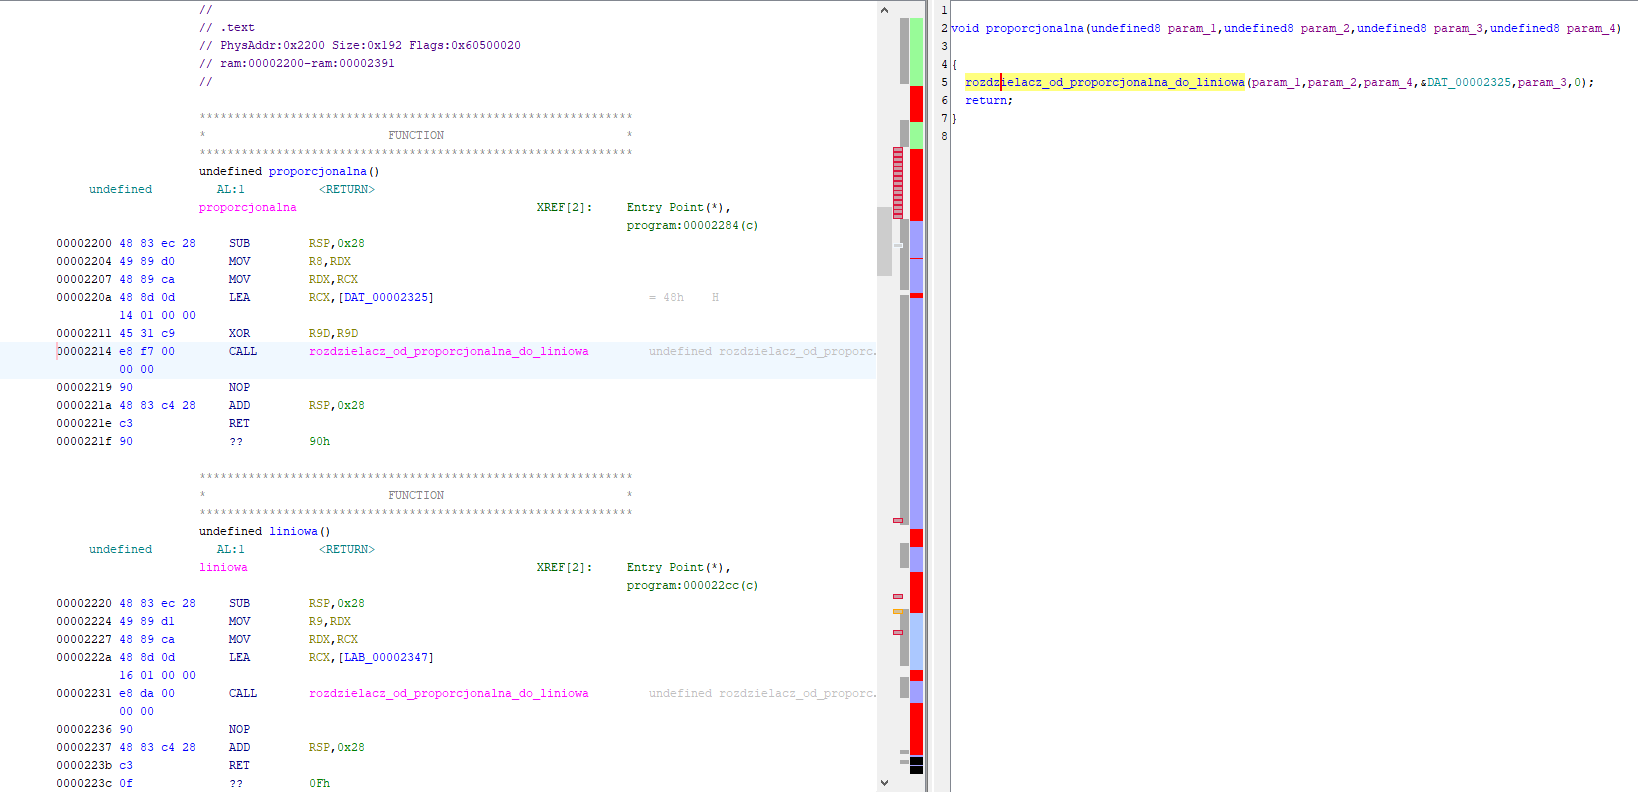
\includegraphics[width=1.2\textwidth]{images/2.rozdzielacz/1.png}
    \caption{Funkcja pośrednicząca}
\end{figure}
\FloatBarrier

Gdy jednak przejdziemy do funkcji rozdzielacza, zobaczymy, że dekompilator nie poradził sobie.
\begin{figure}[H]
    \centering
    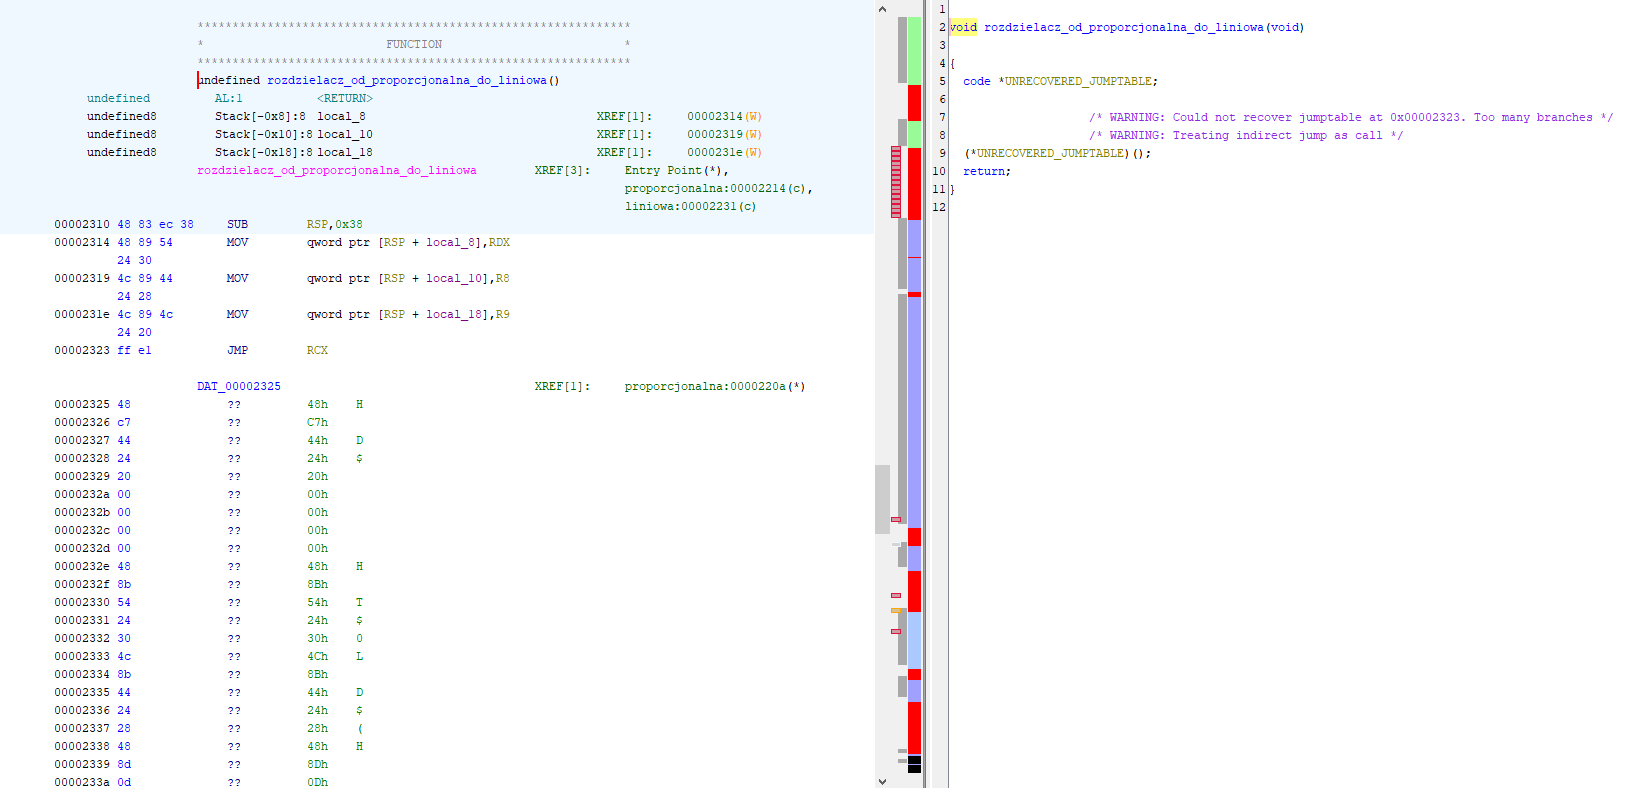
\includegraphics[width=1.2\textwidth]{images/2.rozdzielacz/2.png}
    \caption{Błędnie zdekompilowany rozdzielacz}
\end{figure}

Znajdująca się pod adresem 0002323 instrukcja JMP RCX jest poprawnym tłumaczeniem indirectbr \%0 - ,,skocz do adresu przekazanego w pierwszym parametrze'' w LLVM IR. Jednakże, dekompilator, natrafiając na skok pośredni, spodziewa się najwyraźniej, że jest to część tłumaczenia instrukcji switch i spodziewa się znaleźć tablicę skoków (której w tym wypadku nie potrzebujemy), stąd komunikat ,,Could not recover jumptable''. Nie możemy winić Ghidry za porażkę w tym wypadku, pokazaliśmy przecież wcześniej, że owej konstrukcji nie da się zapisać w C.

Możemy jednak uzyskać widok zdekompilowanego ciała funkcji, ręcznie podmieniając instrukcję - JMP RCX na JMP LAB\_00002325, czyli skok do następnego adresu (co dzieje się w jednej ze ścieżek wykonania programu). 
\FloatBarrier
\begin{figure}[H]
    \centering
    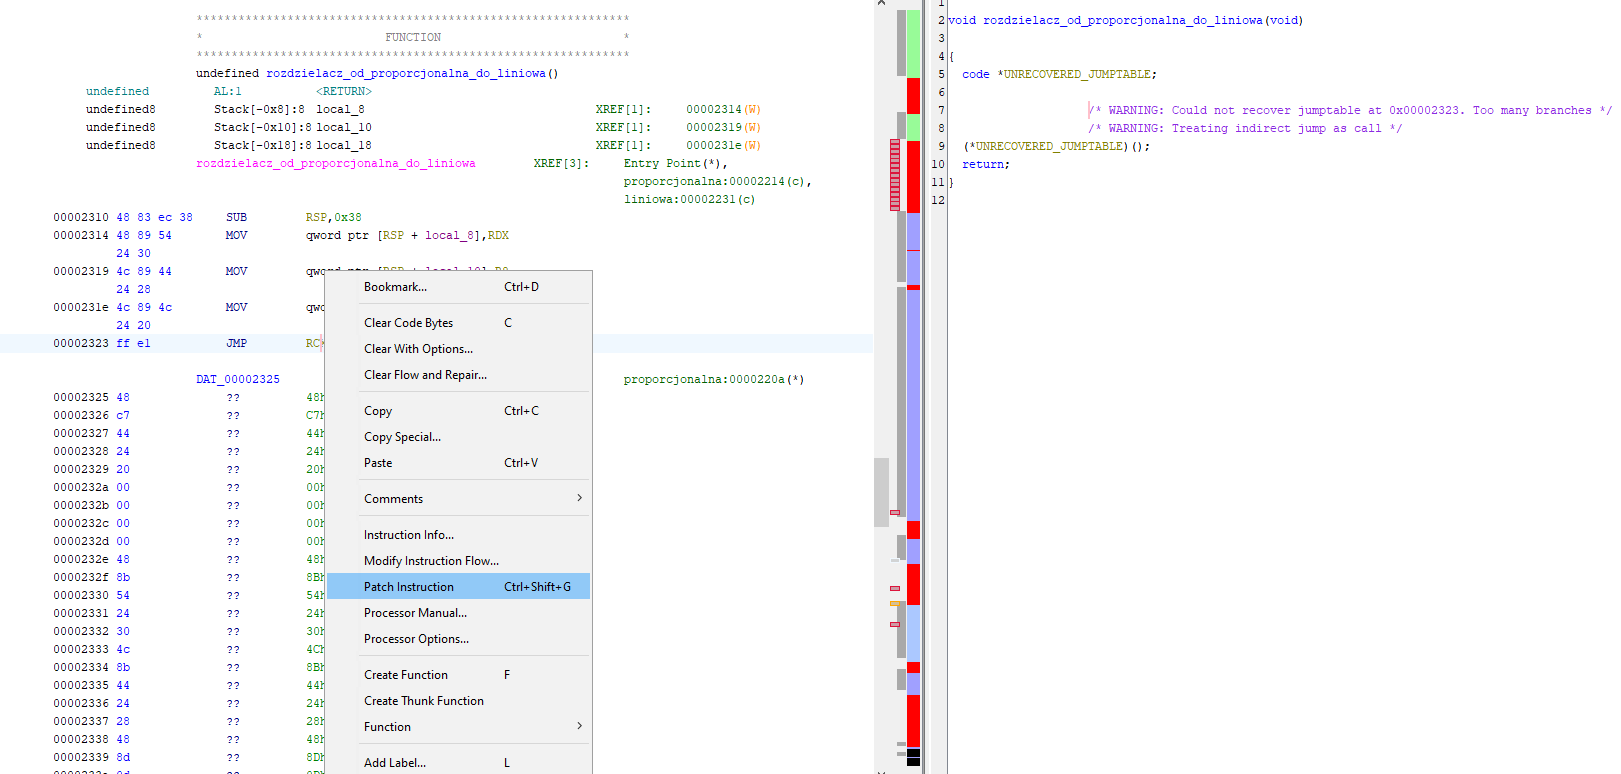
\includegraphics[width=1.2\textwidth]{images/2.rozdzielacz/3.png}
    \caption{Poprawianie pojedynczej instrukcji}
\end{figure}
Widzimy wtedy, że odtworzona została struktura procedury.
\begin{figure}[H]
    \centering
    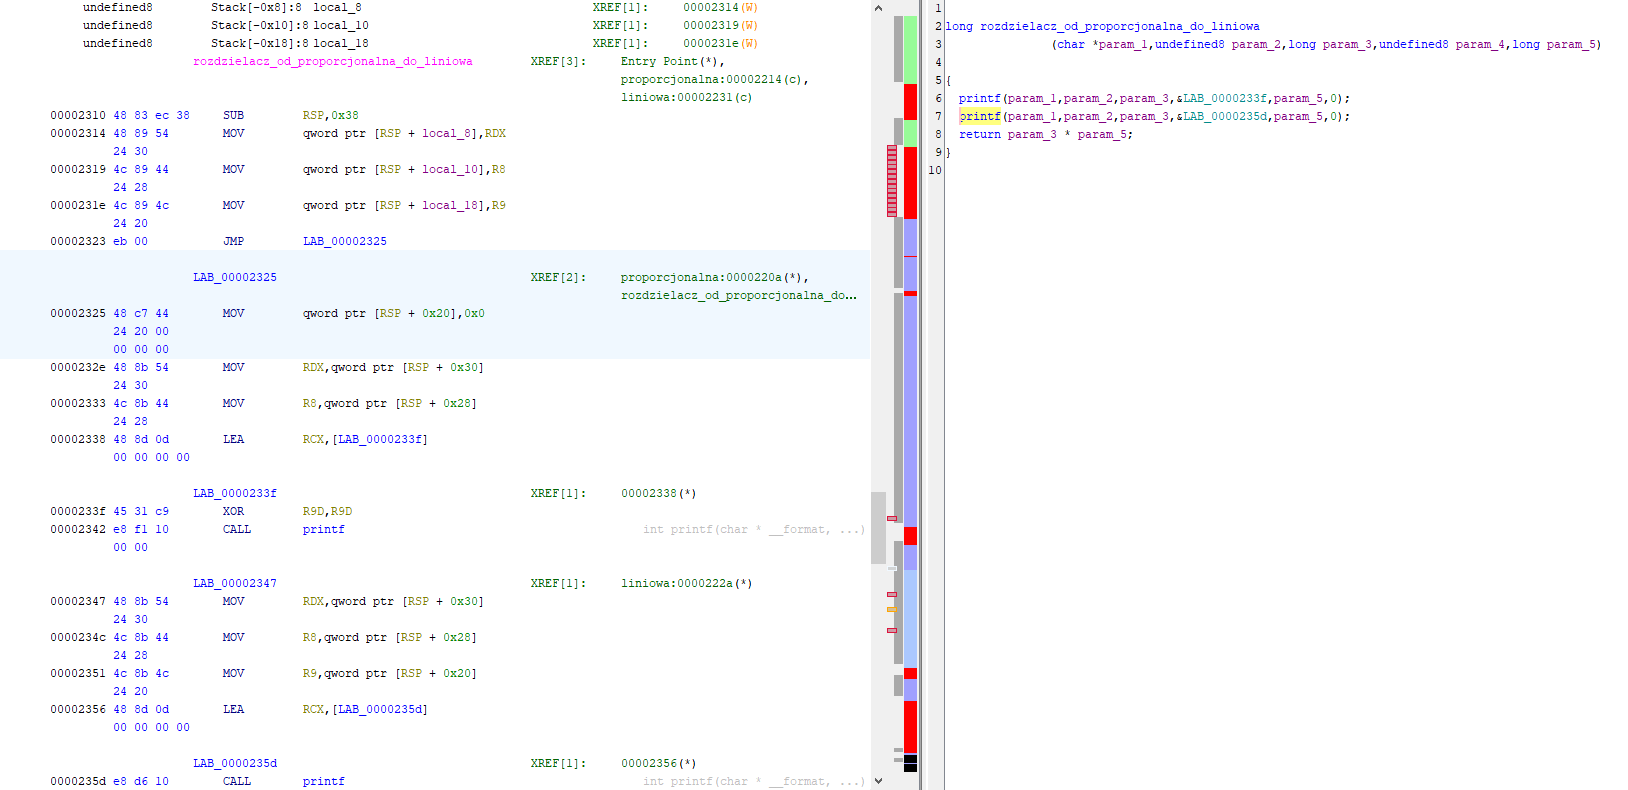
\includegraphics[width=1.2\textwidth]{images/2.rozdzielacz/4.png}
    \caption{Poprawnie zdekompilowany rozdzielacz po podstawieniu jednego z możliwych adresów w instrukcji skoku pośredniego}%%???
\end{figure}

Na sam koniec, sprawdźmy działanie programu (dodając odpowiednie przetwarzanie argumentów wywołania):
\begin{lstlisting}
printf(znak^,...)->całk32;
atoi(znak^)->całk32;
proc {
    zacznij proporcjonalna(całk a, całk x) -> całk;
    całk b=0;
    printf("\nproporcjonalna %lld %lld %lld",a,x,b);
    zacznij liniowa(całk a, całk b, całk x) -> całk;
    printf("\nliniowa %lld %lld %lld",a,x,b);
    zwróć a*x + b;
}
proc { zacznij program(całk argl, znak^^ argw) -> całk;
    całk zwr;
    jeśli(argl == 3)//a x
    {
        zwr = proporcjonalna(atoi(argw[1]), atoi(argw[2]));
    }
    inaczej{
        jeśli(argl == 4)
        {
            zwr = liniowa(atoi(argw[1]), atoi(argw[3]), atoi(argw[2]));
        }inaczej{printf("Zła liczba argumentów:%d a nie 2/3", argl-1); zwróć 0;}
    }
    printf("\nZwraca %d", zwr);
    zwróć 0;
}
\end{lstlisting}

Wywołajmy skompilowany program dwa razy, wchodząc do procedury pierwszym oraz drugim punktem wejściowym.
\begin{figure}[H]
    \centering
    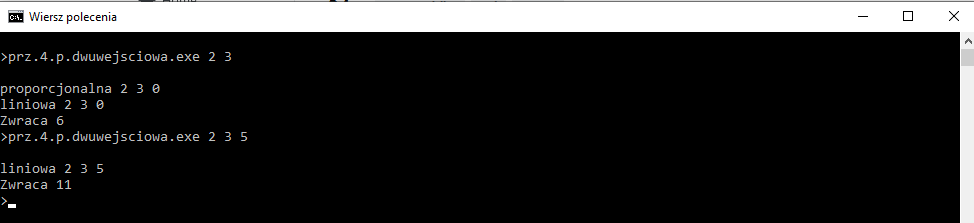
\includegraphics[width=1.0\textwidth]{images/2.rozdzielacz/cmdzrz.png}
    \caption{Dwukrotne wywołanie programu, testując oba punkty wejściowe}
\end{figure}

\section{Przenośność kompilatora}
Używając Javy, nie chciałem jednocześnie zależeć od konkretnego IDE, wybrałem więc Mavena do zarządzania projektem, da się bowiem cały proces budowania uruchomić za pomocą niego samego, z powłoki, powtarzalnie, z potencjałem do automatyzacji.. Wystarczy sklonować projekt z repozytorium i wykonać 'mvn clean install'. Przez wieloplatformowość Javy, oraz to że zależności - przede wszystkim antlr4, llvm i graphviz, są automatycznie pobierane z Sieci (nie jest wymagane instalowanie clanga w systemie), okazało się, że program kompilatora z minimalnymi zmianami w konfiguracji, da się również uruchomić na Linuksie. Rozmiar pobieranych pakietów pozostawia jednak w obecnej wersji wiele do życzenia.
%i to chyba tyle....